\documentclass[compress, color = usenames, dvipsnames]{beamer}

% theme CentraleSupelec
\usepackage{./beamerthemeCS}


% liste de paquets
\usepackage[utf8]{inputenc}
\usepackage[T1]{fontenc}
\usepackage[francais]{babel}
\usepackage{xstring}
\usepackage{hyperref}

% premiere page
\title[Information Systems \& Programming]{Introduction to Information Systems and Programming}
\subtitle[]{\Large \textbf{Course 1 : Python Programming - The Basics}}
\date[SG1 ~-- Gif]{\large SG1 ~-- Gif}
\institute[]{\large CentraleSupélec -- Gif}


%% Introduction :
%% Python fundamentals

%couleur
\definecolor{deepblue}{rgb}{0,0,0.5}
\definecolor{deepred}{rgb}{0.6,0,0}
\definecolor{deepgreen}{rgb}{0,0.5,0}
\definecolor{codegreen}{rgb}{0,0.6,0}
\definecolor{codegray}{rgb}{0.5,0.5,0.5}
\definecolor{codepurple}{rgb}{0.58,0,0.82}
\definecolor{backcolour}{rgb}{0.95,0.95,0.92}
\definecolor{eclipseBlue}{RGB}{42,0.0,255}
\definecolor{eclipseGreen}{RGB}{63,127,95}
\definecolor{eclipsePurple}{RGB}{127,0,85}

\definecolor{myOrange}{RGB}{232,134,6}
\definecolor{myPink}{RGB}{239,21,239}
\definecolor{myMarineGrey}{RGB}{81,92,109}

\definecolor{myGrey}{RGB}{102,102,102}
\definecolor{myDarkYellow}{RGB}{249,227,27}
\definecolor{myDarkGreen}{RGB}{15,130,20}
\definecolor{myDarkBlue}{RGB}{15,50,140}
\definecolor{myDarkRed}{RGB}{120,10,10}

\definecolor{myLightGrey}{RGB}{204,204,204}
\definecolor{myCommentColor}{RGB}{15,130,20}

\definecolor{modernBlue}{HTML}{B5C9D4}
\definecolor{modernOrange}{HTML}{FD7E47}





% Commandes spécifiques

\usepackage{pifont}
\usepackage{textcomp}
\usepackage{textpos}

\newcommand{\ok}{{\green{\ding{51}}}}
\newcommand{\nok}{\orange{\ding{55}}}
\newcommand{\imp}{\blue{\ding{220}}}

\newcommand{\itemOk}{\item[\ok]}
\newcommand{\itemNo}{\item[\nok]}
\newcommand{\itemSo}{\item[\imp]}

% JTO
\usepackage[ruled,vlined]{algorithm2e}
\usepackage{mathrsfs}

% MAWE
\usepackage{listings}
\lstdefinestyle{myPYTHONstyle}{
  language={Python},
  basicstyle=\small\ttfamily, % Global Code Style
  captionpos=b, % Position of the Caption (t for top, b for bottom)
  extendedchars=true, % Allows 256 instead of 128 ASCII characters
  tabsize=4, % number of spaces indented when discovering a tab 
  columns=fixed, % make all characters equal width
  keepspaces=true, % does not ignore spaces to fit width, convert tabs to spaces
  showstringspaces=false, % lets spaces in strings appear as real spaces
  breaklines=false, % wrap lines if they don't fit
  frame=trbl, % draw a frame at the top, right, left and bottom of the listing
  frameround=tttt, % make the frame round at all four corners
  framesep=4pt, % quarter circle size of the round corners
  numbers=left, % show line numbers at the left
  numberstyle=\tiny\ttfamily, % style of the line numbers
  commentstyle=\color{eclipseGreen}, % style of comments
  keywordstyle=\color{eclipseBlue}, % style of keywords
  stringstyle=\color{eclipsePurple}, % style of strings
  numberstyle=\color{codegray},
  xleftmargin=15pt
}


\usepackage{xstring}




\begin{document}



\frame{
  \titlepage
}

\begin{frame}
  \frametitle{Outline}
  \linespread{1.4}
  \tableofcontents[sections={1-4}, subsectionstyle=hide]
\end{frame}

\section[Why Python ?]{The choice of Python as programming language}

\begin{frame}{Python}
\begin{columns}    
\begin{column}{0.7\textwidth}
\begin{block}{A language that is :}
\begin{itemize}
    \item \textbf{Interpreted} (bytecode-compiled),
    \item \textbf{Dynamically and implicitly typed} (no variable declarations),
    \item \textbf{Multi-paradigm} (Imperative, Object-oriented, Functional, Procedural),
    \item with automatic memory management.
\end{itemize}
\end{block}
\end{column}

\begin{column}{0.4\textwidth}
\begin{figure}
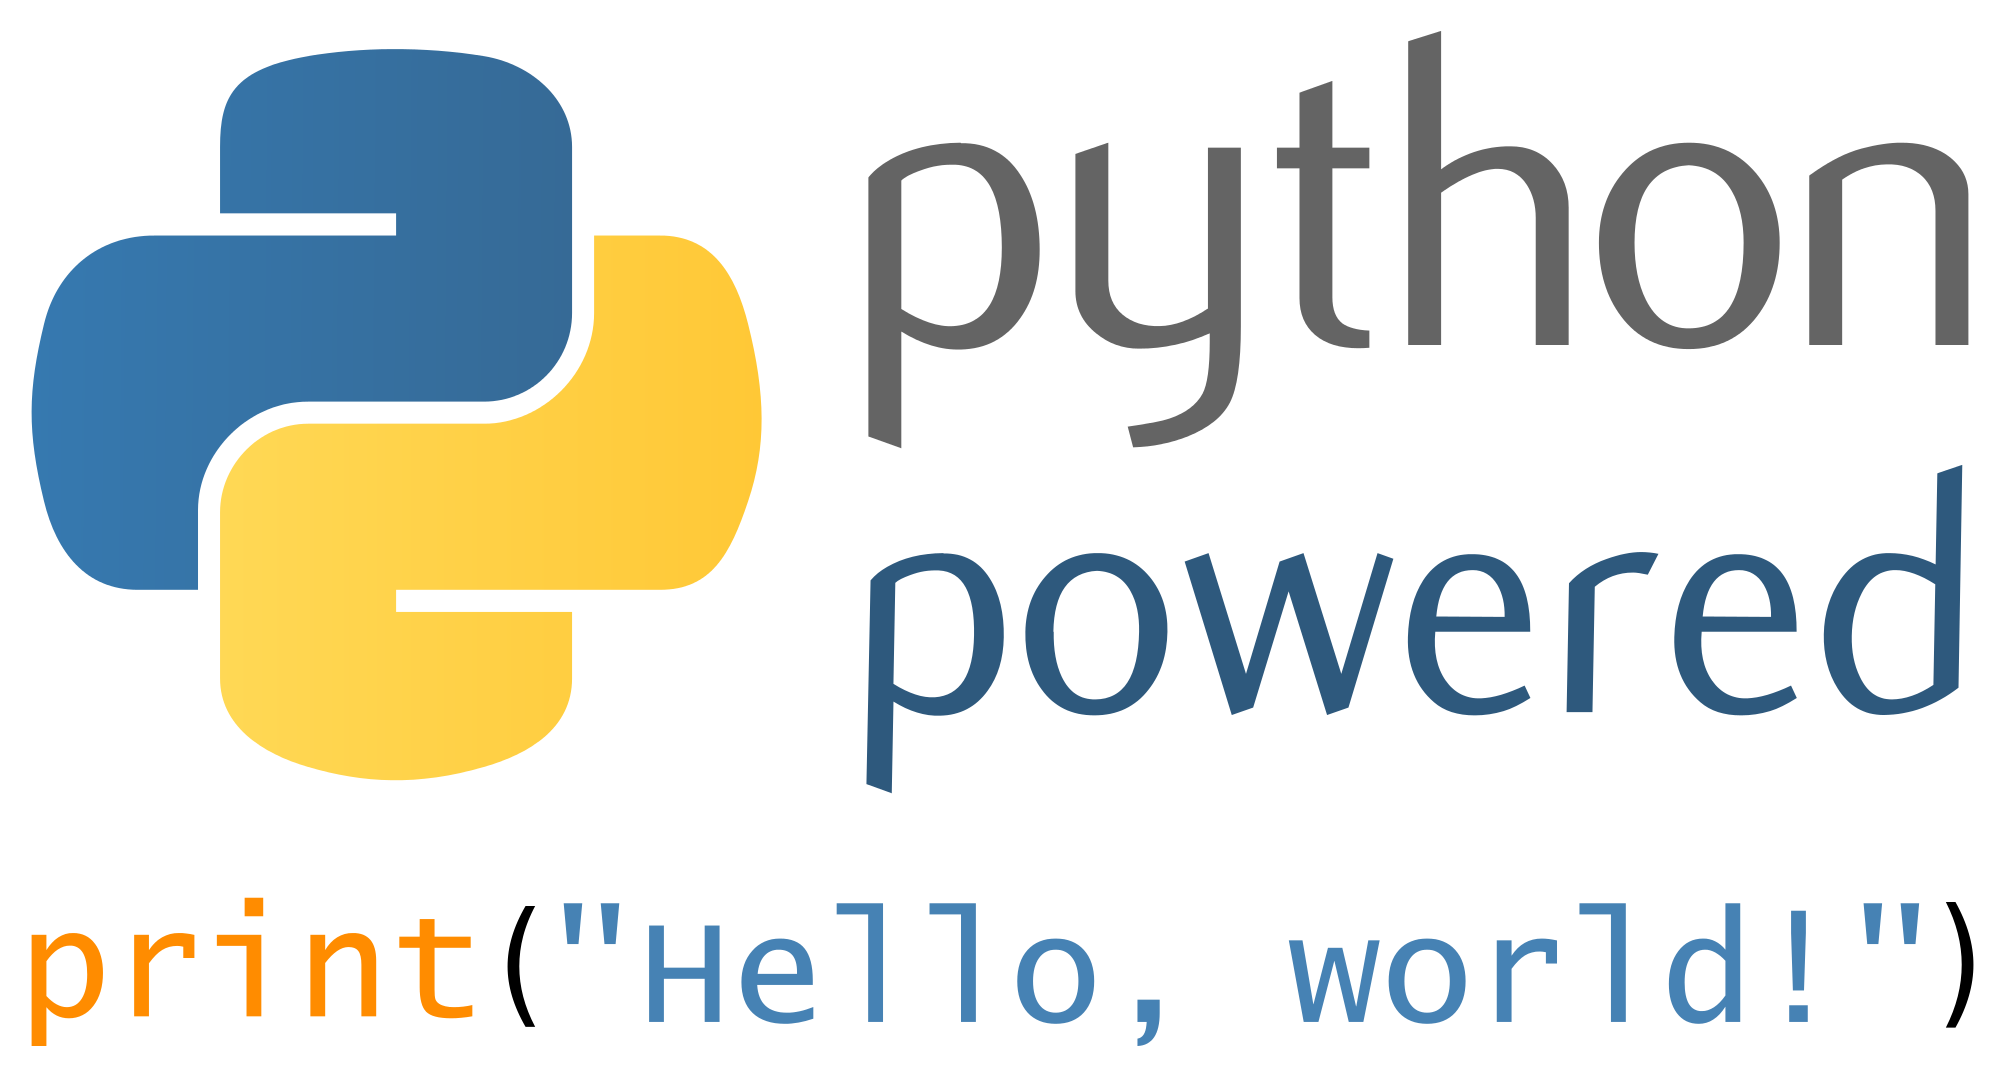
\includegraphics[scale=0.05]{./Images/python.png}
\end{figure}
\end{column}
\end{columns}
\end{frame}
%%%%%%%%%%%%%%%%%%%%%%%%%%%%%%%%%%%%%%%%%%%%%%%%
\begin{frame}{Python}
\begin{columns}    
\begin{column}{0.5\textwidth}
\begin{itemize}
    \item Created by Guido van Rossum\footnote{\url{https://en.wikipedia.org/wiki/Guido_van_Rossum}}
    \item A named derived from the comedy group \textcolor{blue}{Monty Python},
    \item Version 1.0 : 1990.
    \item Version 2.0 : 2000.
    \item \textbf{Version 3.0 : 2008.} \\
    \textcolor{blue}{current version = 3.7.0}
\end{itemize}
\end{column}

\begin{column}{0.5\textwidth}
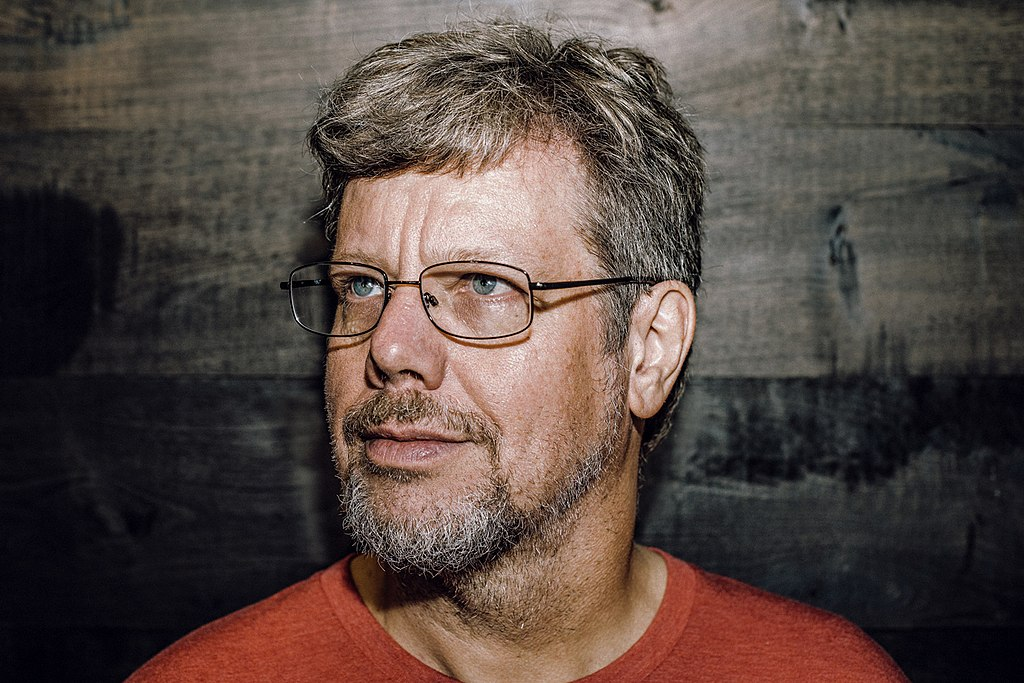
\includegraphics[width=\textwidth]{./Images/guido.jpg}

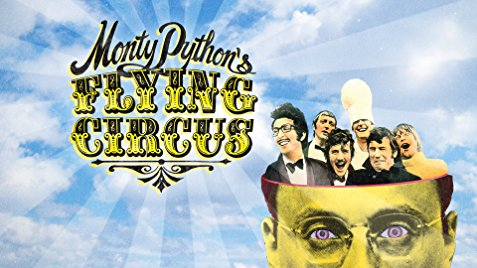
\includegraphics[width=\textwidth]{./Images/monty.jpg}
\end{column}
\end{columns}

\end{frame}
%%%%%%%%%%%%%%%%%%%%%%%%%%%%%%%%%%%%%%%%%%%%%%%%


%%%%%%%%%%%%%%%%%%%%%%%%%%%%%%%%%%%%%%%%%%%%%%%%
\begin{frame}[fragile]{The Zen of Python (by Tim Peters)}
A collection of 20 software principles that influences the design of Python.
\begin{lstlisting}[language=Python,style=myPYTHONstyle]
>>> import this
The Zen of Python, by Tim Peters
\end{lstlisting}



\end{frame}
%%%%%%%%%%%%%%%%%%%%%%%%%%%%%%%%%%%%%%%%%%%%%%%%
\begin{frame}{Documentation}
    
\end{frame}

%%%%%%%%%%%%%%%%%%%%%%%%%%%%%%%%%%%%%%%%%%%%%%%%
\begin{frame}{Your First Program}
\framesubtitle{How to compose and execute a Python program on your system !}
    
\end{frame}


\section[Variables and Types]{Variables and Built-in Types}



\section[Functions]{Funxtions}



\end{document}
